\HeaderQuote{What is the use of a book, without pictures or conversations?}{Alice}

\chapter{Test function suite}\label{app:fun} \todo[color=green!40]{\cref{app:fun} Unfinished}
\FirstSentence{T}{est functions $f$ used} in~\cref{ch:surrogates} are defined $f:\mathbb{R}^d\mapsto\mathbb{R}$.

\todo[inline]{All benchmark functions with the exception of ?? are described in [?]. They are summarized here for completeness. The original sources of the functions are also cited.
\url{https://notendur.hi.is/tpr/software/sres/testfcn.pdf}
}

\section{Sphere }\label{app:fun:sphere}
Sphere function is a convex and unimodal function (cf.~\cref{fig:fun:sphere}). Sphere function is defined as follows,
\begin{eqnarray}
f_{\textrm{Sphere}}(\vec{x})&=&\sum_{i=1}^d x_i^2
\end{eqnarray} where $\vec{x}\in[-3,7]^d$.
It has a global minimum at $\vec{x}=\textbf{0}$ where $f_{\textrm{Sphere}}(\textbf{0})=0$. 

\section{Noisy sphere}\label{app:fun:nsphere}
Noisy sphere function is the sphere function from~\cref{app:fun:sphere} where a Gaussian noise has added to perturb the sphere (cf.~\cref{fig:fun:nsphere} where $\epsilon=0.1$). Noisy sphere function is defined as follows,
\begin{eqnarray}
f_{\textrm{NoisySphere}}(\vec{x})&=&f_{\textrm{Sphere}}(\vec{x})\left(1+\epsilon\mathcal{N}(0,1)\right)
\end{eqnarray} where $\vec{x}\in[-3,7]^d$.
It has a global minimum at $\vec{x}=\textbf{0}$ where $f_{\textrm{NoisySphere}}(\textbf{0})=0$.

\section{Schwefel}\label{app:fun:schwefel}
Schwefel is ... (cf.~\cref{fig:fun:schwefel}). Schwefel function is defined as follows,
\begin{eqnarray}
f_{\textrm{Schwefel}}(\vec{x})&=&\sum_{i=1}^d\left(\sum_{j=1}^i x_j\right)^2
\end{eqnarray} where $\vec{x}\in[-10,10]^d$.
It has a global minimum at $\vec{x}=\textbf{0}$ where $f_{\textrm{Schwefel}}(\textbf{0})=0$.

\section{Ellipsoid}\label{app:fun:ellipsoid}
Ellipsoid is ... (cf.~\cref{fig:fun:ellipsoid}). Ellipsoid function is defined as follows,
\begin{eqnarray}f_{\textrm{Ellipsoid}}(\vec{x})=\sum_{i=1}^d \left(100^{\frac{i-1}{d-1}}x_i\right)^2
\end{eqnarray} where $\vec{x}\in[-3,7]^d$.
It has a global minimum at $\vec{x}=\textbf{0}$ where $f_{\textrm{Ellipsoid}}(\textbf{0})=0$.

\section{Rosenbrock}\label{app:fun:rosen}
Rosenbrock function is a non-convex function, where the global minimum is inside a long, narrow, parabolic shaped flat valley (cf.~\cref{fig:fun:rosen}). To find the valley is trivial. To converge to the global minimum, however, is difficult. Rosenbrock function is defined as follows,
\begin{eqnarray}
f_{\textrm{Rosenbrock}}(\vec{x})&=&\sum_{i=1}^{d-1} \left(100\cdot(x_i^2-x_{i+1})^2+(x_i-1)^2\right)
\end{eqnarray} where $\vec{x}\in[-5,5]^d$. 
It has a global minimum at $\vec{x}=\textbf{1}$ where $f_{\textrm{Rosenbrock}}(\textbf{1})=0$.

\section{Ackley}\label{app:fun:ackley}
Ackley function is a non-convex function, where the function is a fairly difficult problem due to its large search space and its large number of local minima (cf.~\cref{fig:fun:ackley}). Ackley function is defined as follows,
\begin{eqnarray}
f_{\textrm{Ackley}}(\vec{x})&=&20-20\cdot\exp\left(-0.2\sqrt{\frac{1}{n}\sum_{i=1}^d x_i^2}\right)
\\&&+e-\exp\left(\frac{1}{2}\sum_{i=1}^d \cos(2\pi x_i)\right) \nonumber
\end{eqnarray} where $\vec{x}\in[1,30]^d$.
It has a global minimum at $\vec{x}=\textbf{0}$ where $f_{\textrm{Ackley}}(\textbf{0})=0$.

\section{Rastrigin}\label{app:fun:rastrigin}
Rastrigin function is based on the sphere function from~\cref{app:fun:sphere} with the addition of cosine modulation in order to produce frequent local minima (cf.~\cref{fig:fun:rastrigin}). Thus, the test function is highly multimodal. However, the location of the minima are regularly distributed. Rastrigin function is defined as follows,
\begin{eqnarray}
f_{\textrm{Rastrigin}}(\vec{x})&=&10n+\sum_{i=1}^d \left(x_i^2-10\cos(2\pi x_i)\right)
\end{eqnarray} where $\vec{x}\in[1,5]^d$. 
It has a global minimum at $\vec{x}=\textbf{0}$ where $f_{\textrm{Rastrigin}}(\textbf{0})=0$.

\begin{figure}\centering
\subfloat[Sphere function]{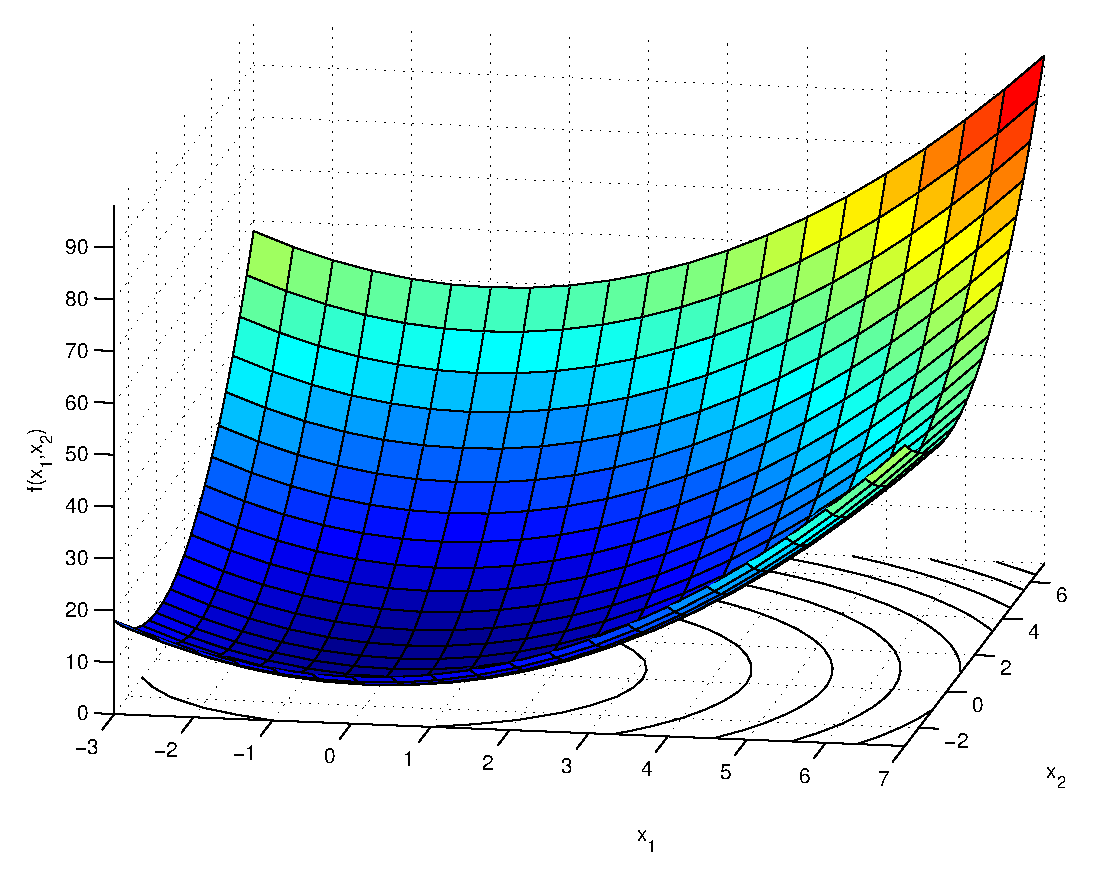
\includegraphics[width=0.37\textwidth]{fun/sphere}\label{fig:fun:sphere}}
\quad
\subfloat[Noisy sphere (with $\epsilon=0.1$)]{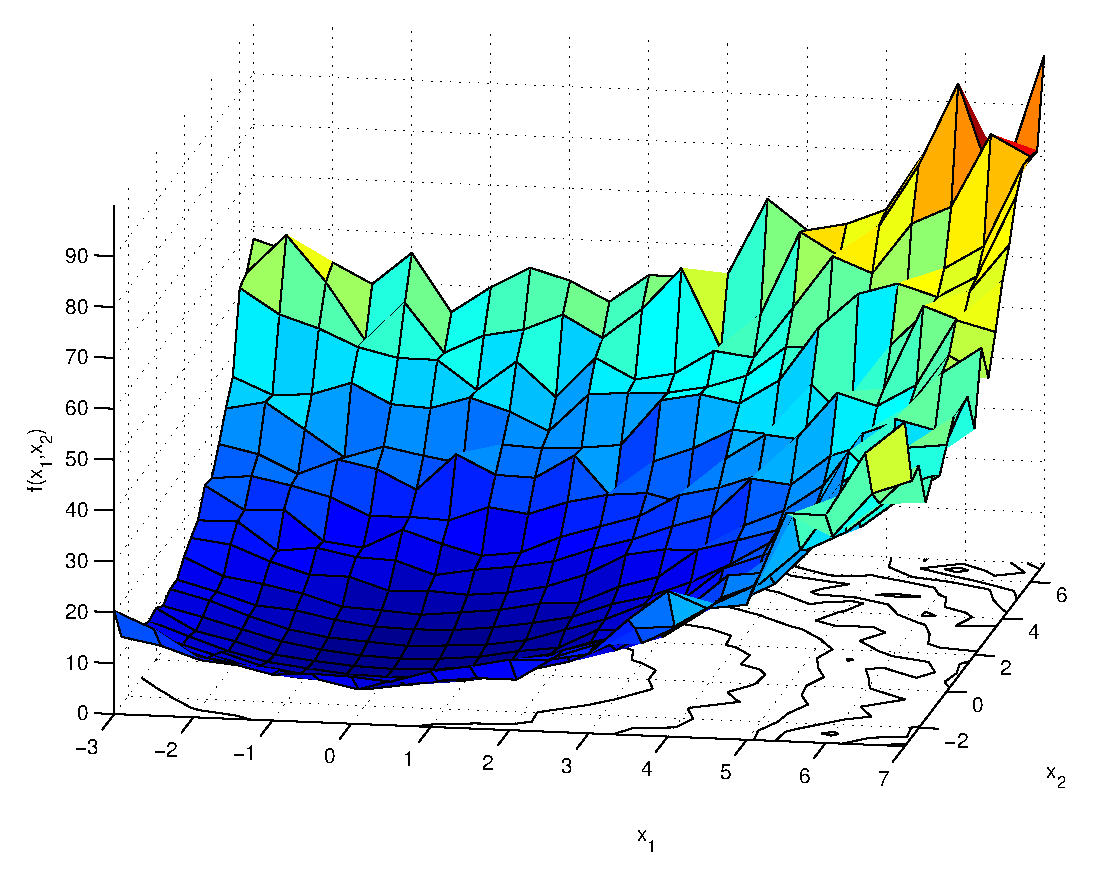
\includegraphics[width=0.37\textwidth]{fun/nsphere}\label{fig:fun:nsphere}}
\\
\subfloat[Schwefel]{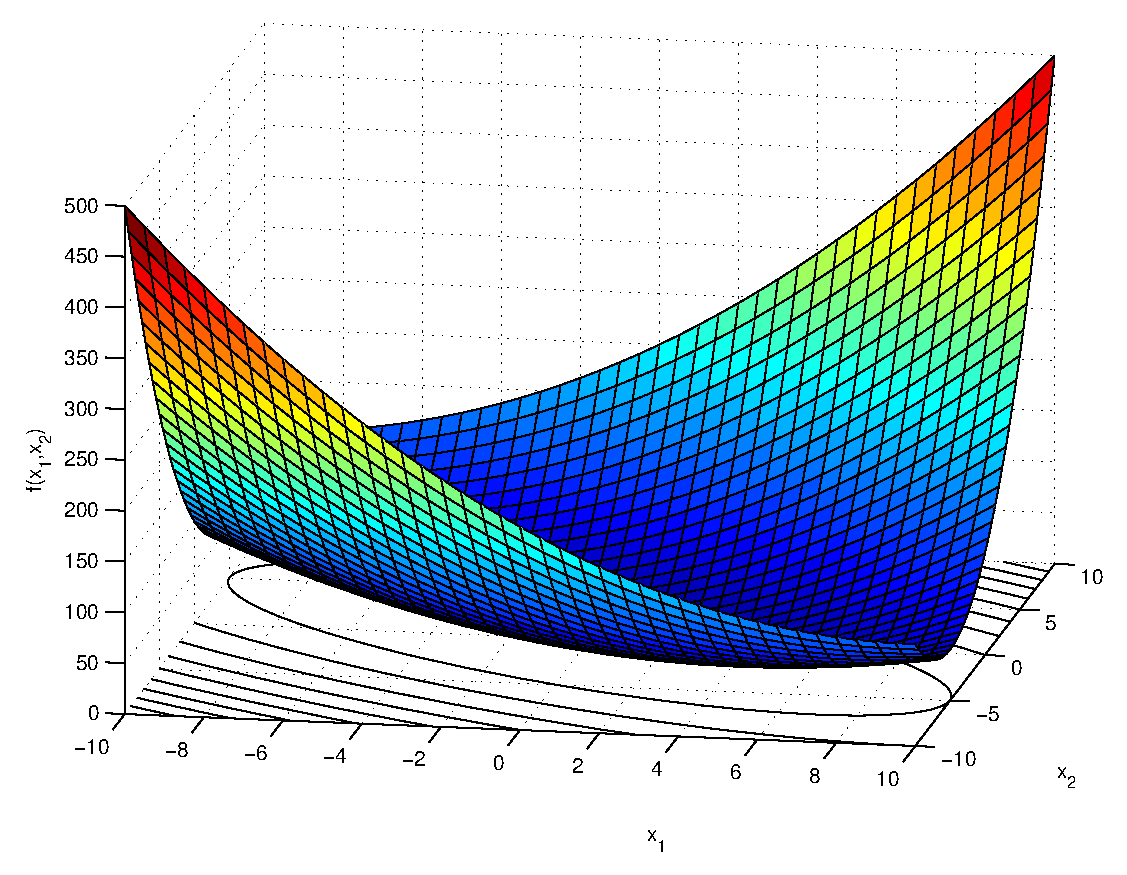
\includegraphics[width=0.37\textwidth]{fun/schwefel}\label{fig:fun:schwefel}}
\quad
\subfloat[Ellipsoid]{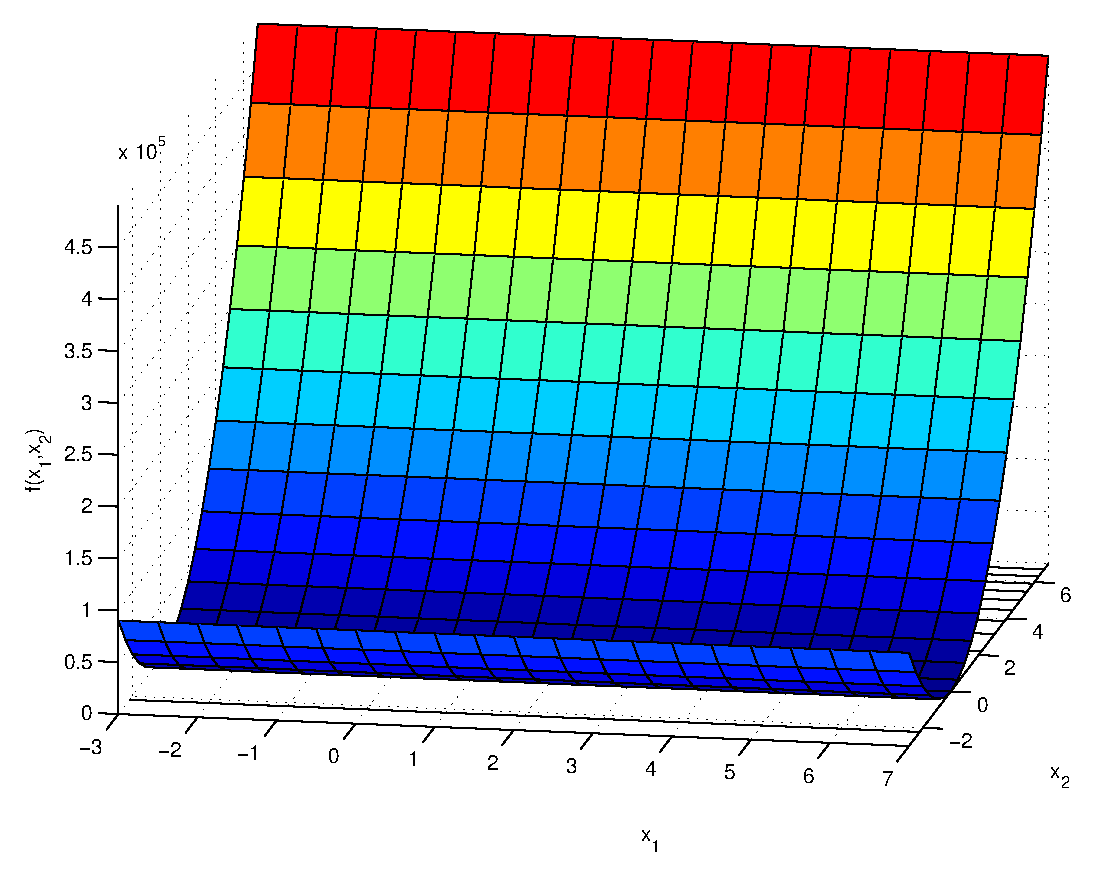
\includegraphics[width=0.37\textwidth]{fun/ellipsoid}\label{fig:fun:ellipsoid}}
\\
\subfloat[Rosenbrock]{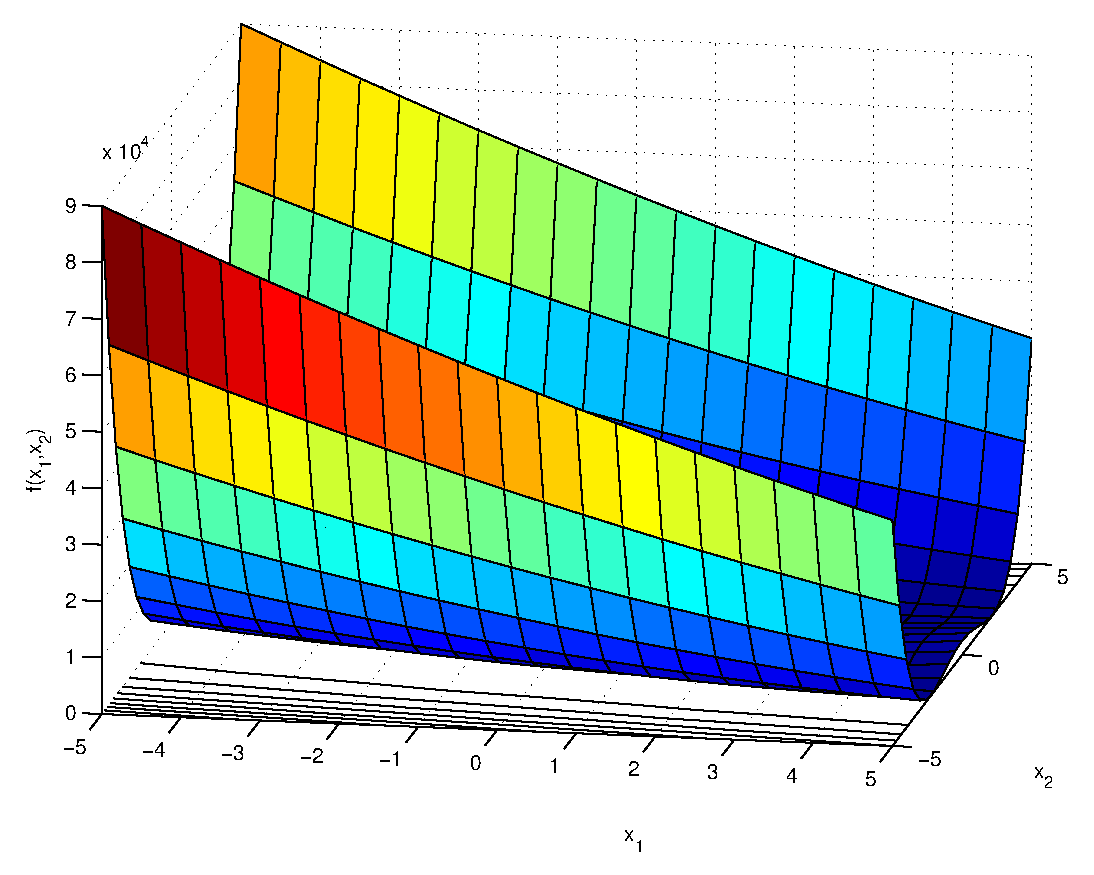
\includegraphics[width=0.37\textwidth]{fun/rosen}\label{fig:fun:rosen}}
\quad
\subfloat[Ackley]{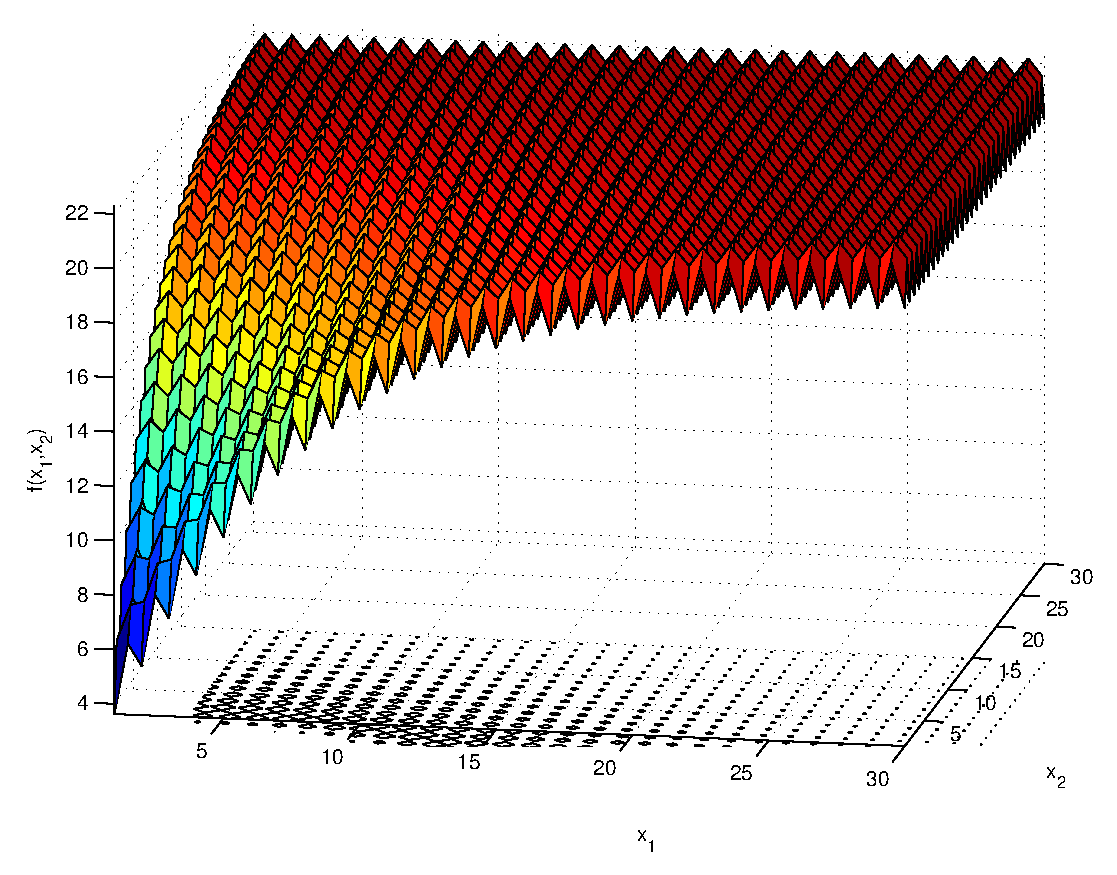
\includegraphics[width=0.37\textwidth]{fun/ackley}\label{fig:fun:ackley}}
\\
\subfloat[Rastrigin]{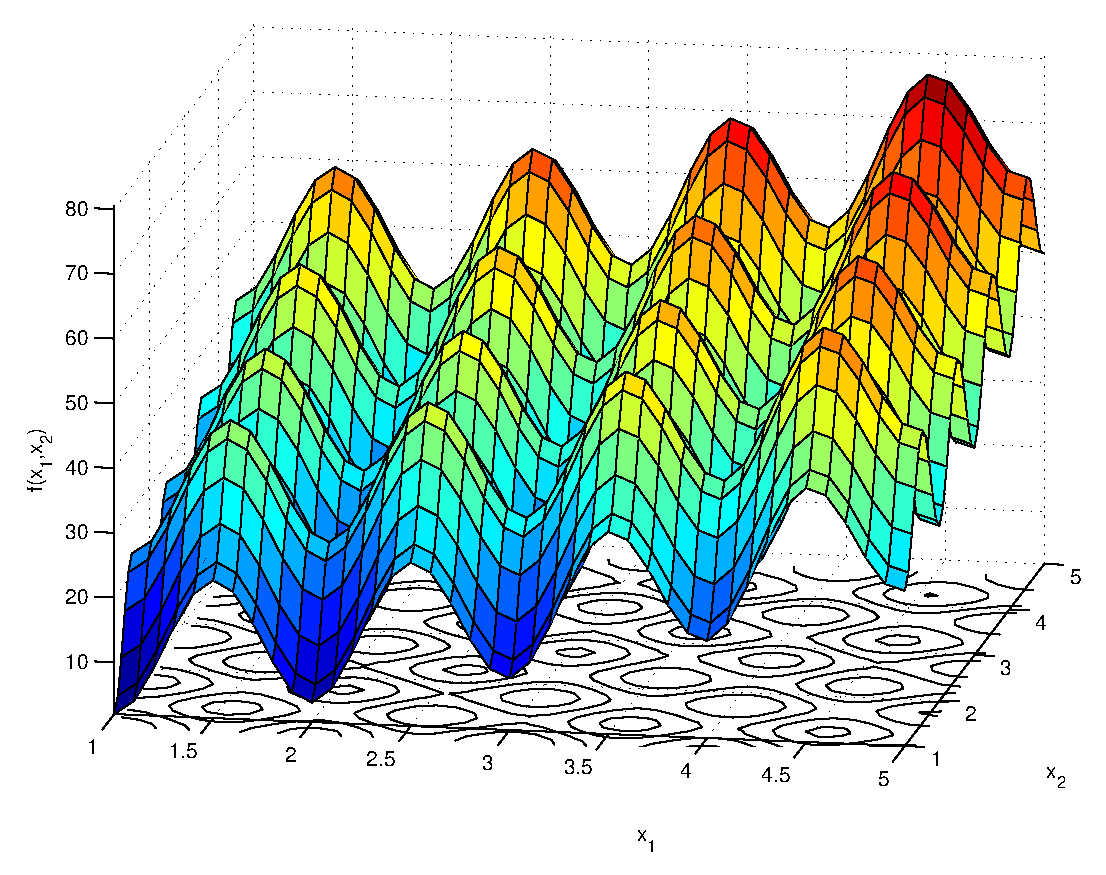
\includegraphics[width=0.37\textwidth]{fun/rastrigin}\label{fig:fun:rastrigin}}
\caption{Test function suite of two variables in 3D.}
\end{figure}





